\newpage

%%%%%%%%%%%%%%%%%%%%  解答（旧 prob_p117〜p120_1.png）  %%%%%%%%%%%%%%%%%%%%
\setlength{\columnseprule}{0.4pt}
\begin{multicols}{2}
\raggedcolumns

{\gtfamily\large 第14回　気体の状態方程式・\\ 熱力学第一法則}\par\vspace{2mm}

\Rank{A問題}
\MonN{1}{基本事項の確認}\par\nopagebreak
\begin{sisin}
状態方程式$PV=nRT$や圧力と力の関係式$F=PS$などの関係式を利用せよ．
\end{sisin}
\noindent{\gtfamily 【解答】}\par\nopagebreak
\begin{komon}
\ko{1} $P=\dfrac{F}{S}=\dfrac{5.0}{1.0\times 10^{-2}}=5.0\times 10^2\U{Pa}$\Ans
\ko{2} $\mathrm{O_2}$の分子量は$M=32\U{g/mol}$なので，$96\U{g}$は$n=\dfrac{w}{M}=\dfrac{96}{32}=3.0\U{mol}$に相当．よって，分子数は
       \[N=n\cdot N_{\mathrm{A}}=3.0\times 6.02\times 10^{23}\]
       \hspace*{2zw}$\fallingdotseq 1.8\times 10^{24}$\,[個]\Ans
\ko{3} 水の比熱は$1\U{cal/g\cdot K}$であるから，
       \[Q=mc\Delta t=300\cdot 1\cdot(100-20)\]
       \hspace*{2zw}$=2.4\times 10^4\U{cal}$\par
       また，$1\U{cal}=4.2\U{J}$なので，
       \[Q=2.4\times 10^4\times 4.2\U{J}\fallingdotseq 1.0\times 10^5\U{J}\Ans\]
\ko{4} $Q=mc\Delta t$より，$56000=200\times c\times(60-20)$が成り立つから，
       \[c=\frac{56000}{200\cdot(60-20)}=7.0\U{cal/g\cdot K}\]
       また，熱容量は，
       \[C=m\cdot c=7.0\times 200\]
       \hspace*{2zw}$=1.4\times 10^3\U{cal/K}$\Ans
\end{komon}

\Rank{B問題}
\MonN{2}{状態方程式}\par\nopagebreak
\begin{sisin}
状態方程式$PV=nRT$を元にして考える．ある量を固定して他の量を変化させる場合には，左辺もしくは右辺に変化しない量をまとめてしまうのがコツである．例えば(2)の変化では，気体の圧力が一定なので，状態方程式で一定の量の$n$, $R$, $p$を右辺にまとめると，$\dfrac{V}{T}=\dfrac{nR}{p}=$（一定）となり，$\dfrac{V}{T}$が変化していないことが分かる．
\end{sisin}
\noindent{\gtfamily 【解答】}\par\nopagebreak
\hspace{1zw}気体が$n\U{mol}$あるとする．また，気体定数を$R\U{J/mol\cdot K}$とする．
\begin{komon}
\ko{1} この状態変化では気体の温度が一定であるから，理想気体の状態方程式の$n$, $R$, $T$が一定に保たれる．よって状態方程式より，$pV=nRT=$（一定）となる．変化後の気体の圧力を$p'\U{Pa}$とすれば，
       \[p'\cdot kV_0=p_0\cdot V_0\]
       ゆえに，
       \[p'=\frac{1}{k}p_0\U{Pa}\Ans\]
\ko{2} この状態変化では気体の圧力が一定であるから，理想気体の状態方程式の$n$, $R$, $p$が一定に保たれる．よって状態方程式より，$\dfrac{V}{T}=\dfrac{nR}{p}=$（一定）となる．変化後の気体の体積を$V'\U{m^3}$とすれば，
       \[\frac{V'}{kT_0}=\frac{V_0}{T_0}\]
       ゆえに，
       \[V'=kV_0\U{m^3}\Ans\]
\ko{3} この状態変化では気体の体積が一定であるから，理想気体の状態方程式の$n$, $R$, $V$が一定に保たれる．よって状態方程式より，$\dfrac{p}{T}=\dfrac{nR}{V}=$（一定）となる．変化後の気体の温度を$T'\U{K}$とすれば，
       \[\frac{kp_0}{T'}=\frac{p_0}{T_0}\]
       ゆえに，
       \[T'=kT_0\U{K}\Ans\]
\ko{4} この状態変化においては圧力，体積，温度が変化するので状態方程式をそのまま利用する．始めの状態の状態方程式は，
       \[p_0V_0=nRT_0\]
       変化後の状態方程式は，絶対温度が$t_1+273.15\U{K}$であることに注意して，変化後の体積を$V_1\U{m^3}$とすると，
       \[p_1V_1=nR(t_1+273.15)\]
       以上2式から$n$, $R$を消して$V_1$を求めると，
       \[V_1=\frac{p_0(t_1+273.15)}{p_1T_0}V_0\U{m^3}\Ans\]
\end{komon}
\begin{chuu}
\hspace{1zw}上の解答では状態方程式を変形することで答えを導いたが，(4)と同様に，変化前・変化後の二つの状態方程式から答えを導いてもよい．例えば(2)であれば，変化前の状態方程式$p_0V_0=nRT_0$と，変化後の状態方程式$p_0V'=nR(kT_0)$の二つの組み合わせから，$V'=kV_0\U{m^3}$を導くことが可能である．
\end{chuu}

\MonN{3}{状態方程式}\par\nopagebreak
\begin{sisin}
ピストン$\mathrm{C}$は$\mathrm{A}$，$\mathrm{B}$の気体から圧力を受けるが，例えば$\mathrm{A}$からの圧力の方が大きければピストンは右へ移動する．よって，ピストンが静止しているときは$\mathrm{A}$，$\mathrm{B}$の圧力は等しい．また，$\mathrm{C}$は断熱材であるから，$\mathrm{A}$，$\mathrm{B}$の温度は等しくなくてもよい．

本問のような問題では，変化前・変化後の気体の状態方程式を立てて考えるのが基本である．問題文では状態方程式を立てるのに必要な変数がすべて与えられていないので，適宜仮定した上で状態方程式を立てよう．
\end{sisin}
\noindent{\gtfamily 【解答】}\par\nopagebreak
\hspace{1zw}ピストン$\mathrm{C}$の断面積を$S\U{m^2}$，$\mathrm{A}$，$\mathrm{B}$内の気体の物質量を$n_{\mathrm{A}}\U{mol}$，$n_{\mathrm{B}}\U{mol}$とし，気体定数を$R\U{J/mol\cdot K}$とすると，最初の状態についての状態方程式より，
\[\mathrm{A}:p_0(Sl_{\mathrm{A}})=n_{\mathrm{A}}RT_0\Eq{1}\]
\[\mathrm{B}:p_0(Sl_{\mathrm{B}})=n_{\mathrm{B}}RT_0\Eq{2}\]
である．
\begin{komon}
\ko{1} $\mathrm{B}$内の気体の温度を上げると，$\mathrm{B}$内の気体の圧力の方が$\mathrm{A}$内の気体の圧力より大きくなってしまうので，ピストン$\mathrm{C}$は$\mathrm{B}$から$\mathrm{A}$の向きへ移動する．\Ans
\ko{2} ピストン$\mathrm{C}$は自由に動くことができるので，ピストン$\mathrm{C}$が移動して静止した時の$\mathrm{A}$，$\mathrm{B}$内の気体の圧力は等しい．これを$p\U{Pa}$とする．また，このときの$\mathrm{A}$内の気体の温度を$T\U{K}$とすると，変化後のシリンダーの長さがそれぞれ$l_{\mathrm{A}}-l$, $l_{\mathrm{B}}+l$になっていることに注意して，
       \[\mathrm{A}:p\cdot S(l_{\mathrm{A}}-l)=n_{\mathrm{A}}RT\Eq{3}\]
       \[\mathrm{B}:p\cdot S(l_{\mathrm{B}}+l)=n_{\mathrm{B}}RT_1\Eq{4}\]
       が成立する．これと先に立てた状態方程式を組み合わせる．\MARU{2}，\MARU{4}より，
       \[p=\frac{l_{\mathrm{B}}T_1}{(l_{\mathrm{B}}+l)T_0}p_0\U{Pa}\Ans\]
       また，\MARU{1}，\MARU{3}および$p$より，
       \[T=\frac{(l_{\mathrm{A}}-l)l_{\mathrm{B}}}{(l_{\mathrm{B}}+l)l_{\mathrm{A}}}T_1\U{K}\Ans\]
\end{komon}
\begin{chuu}
\hspace{1zw}$\mathrm{A}$内の気体の温度が変化することに注意．
\[\mbox{「熱の出入りがない」}\]
\[=\mbox{「温度が変化しない」}\]
と考えるのは間違いである．
\end{chuu}

\MonN{4}{熱量の保存}\par\nopagebreak
\begin{sisin}
一般的に，熱は温度の高いものから低いものへと移っていき，最終的には両者の温度が等しくなって熱の移動が止まる．この状態を「熱平衡状態」と呼ぶ．

熱量の保存より，$\mathrm{A}$が失った熱量分を$\mathrm{B}$が受け取っている．よって，熱平衡状態の温度を適当な文字でおき，$\mathrm{A}$が失った熱量と$\mathrm{B}$が得た熱量をその文字で表して考える．
\end{sisin}
\noindent{\gtfamily 【解答】}\par\nopagebreak
\begin{komon}
\ko{1} 熱平衡状態における$\mathrm{A}$，$\mathrm{B}$の温度を$t\U{C}$とする．この状態に至るまでに，$\mathrm{A}$の温度は$t_{\mathrm{A}}-t$だけ下がり，$\mathrm{B}$の温度は$t-t_{\mathrm{B}}$だけ上がる．よって$\mathrm{A}$が失った熱量$Q_{\mathrm{A}}\U{cal}$および$\mathrm{B}$が得た熱量$Q_{\mathrm{B}}\U{cal}$は，
       \[Q_{\mathrm{A}}=m_{\mathrm{A}}c_{\mathrm{A}}(t_{\mathrm{A}}-t),\]
       \[Q_{\mathrm{B}}=m_{\mathrm{B}}c_{\mathrm{B}}(t-t_{\mathrm{B}})\]
       \hspace{1zw}熱量の保存より，$\mathrm{A}$が失った熱量と$\mathrm{B}$が得た熱量は等しいので，
       \[m_{\mathrm{A}}c_{\mathrm{A}}(t_{\mathrm{A}}-t)=m_{\mathrm{B}}c_{\mathrm{B}}(t-t_{\mathrm{B}})\]
       である．これを解いて，
       \[t=\frac{m_{\mathrm{A}}c_{\mathrm{A}}t_{\mathrm{A}}+m_{\mathrm{B}}c_{\mathrm{B}}t_{\mathrm{B}}}{m_{\mathrm{A}}c_{\mathrm{A}}+m_{\mathrm{B}}c_{\mathrm{B}}}\U{C}\Ans\]
\ko{2} (1)の$t$を$Q_{\mathrm{A}}$, $Q_{\mathrm{B}}$の式に代入して，
       \[Q_{\mathrm{A}}=Q_{\mathrm{B}}=\frac{m_{\mathrm{A}}c_{\mathrm{A}}m_{\mathrm{B}}c_{\mathrm{B}}(t_{\mathrm{A}}-t_{\mathrm{B}})}{m_{\mathrm{A}}c_{\mathrm{A}}+m_{\mathrm{B}}c_{\mathrm{B}}}\U{cal}\]
       \hspace*{\fill}\Ans
\end{komon}

\MonN{5}{熱量の保存}\par\nopagebreak
\begin{sisin}
最終的に全体の温度が$t'\U{C}$になったのであるから，水，銅球だけでなく容器の温度も変化している．熱の移動を考えれば，銅球が失った熱量は水，容器の温度上昇に利用されている．これを表す式を立てればよい．
\end{sisin}
\noindent{\gtfamily 【解答】}\par\nopagebreak
\hspace{1zw}銅の比熱を$c\U{cal/g\cdot K}$とする．この変化にて銅球は$t-t'$だけ温度が下がり，水と容器はともに$t'-t_0$だけ温度が上がったので，銅球が失った熱量$Q\U{cal}$，水，熱量計が得た熱量$Q'\U{cal}$，$Q''\U{cal}$はそれぞれ，
\[Q=mc(t-t')\]
\[Q'=w\cdot 1\cdot(t'-t_0)\]
\hspace*{2zw}（注：水の比熱は$1\U{cal/g\cdot K}$）
% 誤植訂正（2026-08-29）：元の問題集はこの注が Q''=Mc(t'-t_0) の行に置かれていたが，
%   注が説明しているのは Q' の式に現れる「1」（水の比熱）なので Q' の行に移した．
%   Q'' は銅製の容器の式で，比熱は c であり 1 ではない．
\[Q''=Mc(t'-t_0)\]
\hspace{1zw}熱量の移動を考えると，銅球が失った熱量が，水と容器の温度上昇に利用されたので，
\[Q=Q'+Q''\]
以上をまとめると，
\[c=\frac{w(t'-t_0)}{m(t-t')-M(t'-t_0)}\U{cal/g\cdot K}\]
\hspace*{\fill}\Ans

\MonN{6}{摩擦熱}\par\nopagebreak
\begin{sisin}
自動車がブレーキをかけると摩擦力の作用により車は静止する．これをエネルギー的な観点から見ると，摩擦力によって自動車の持っていた力学的エネルギーが減少し，その減少分は熱として空気中などに散逸している．この熱を\underline{摩擦熱}という．最終的に静止したのだから，持っていた運動エネルギーすべてが摩擦熱に転化したことになる．

また運動エネルギーを求める際には，まず速さ，質量をMKS単位系に直してエネルギーを$\U{J}$単位で求めよう．
\end{sisin}
\noindent{\gtfamily 【解答】}\par\nopagebreak
\hspace{1zw}ブレーキをかける前に自動車がもっていた運動エネルギーを$E\U{J}$とする．
\[1\U{t}=1000\U{kg}\]
\[72\U{km/h}=\frac{72000\U{m}}{3600\U{s}}=20\U{m/s}\]
であるから，
\[E=\frac{1}{2}mv^2=\frac{1}{2}\cdot 1000\cdot 20^2\]
\hspace*{2zw}$=2.0\times 10^5\U{J}$\par
\hspace{1zw}摩擦によって失われた運動エネルギーはすべて摩擦熱となったので，このとき生じた熱量は$2.0\times 10^5\U{J}$である．これを$\U{cal}$単位に換算して，
\[Q=\frac{2.0\times 10^5}{4.2}\fallingdotseq 4.8\times 10^4\U{cal}\Ans\]

\MonN{7}{熱力学第一法則}\par\nopagebreak
\begin{sisin}
熱力学第一法則を考える際には，熱量，仕事の出入りを把握するのが第一である．それを把握したら，簡単な図を描いてエネルギー収支を日本語で考え，それを式として表せばよい．

熱や仕事のやり取りを，気体に対して加えられたとみなして考えた場合と，気体が外界に対して放出したとみなして考えた場合とは，正負が逆になる．
\end{sisin}
\noindent{\gtfamily 【解答】}\par\nopagebreak
\begin{komon}
\ko{1} 外部が気体に与えた熱量は$Q$，外部が気体にした仕事は$-W$，気体の内部エネルギーの増加量は$\Delta U$であるから，
       \[\Delta U=Q+(-W)\Ans\]
       \begin{center}
       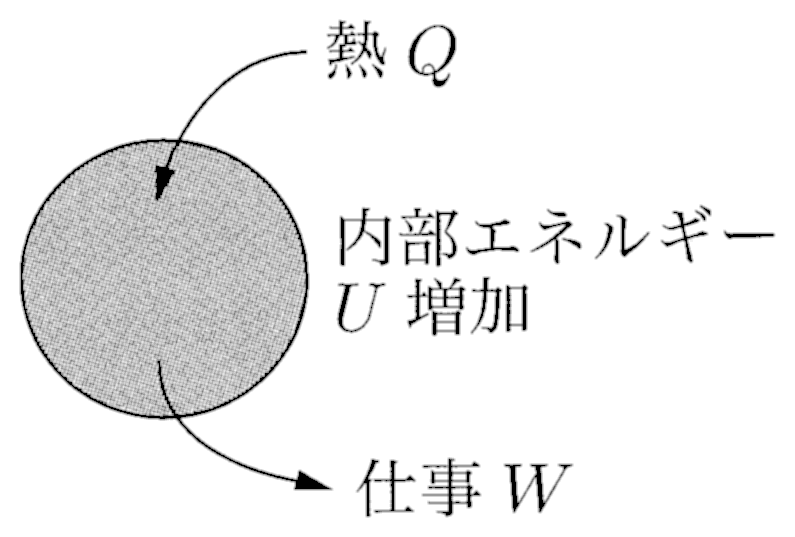
\includegraphics[keepaspectratio,width=38mm]{fig/ch14_p119_dU1.png}
       \end{center}
\ko{2} 外部が気体に与えた熱量は$-Q'$，外部が気体にした仕事は$W'$，気体の内部エネルギーの増加量は$\Delta U$であるから，
       \[\Delta U=(-Q')+W'\Ans\]
       \begin{center}
       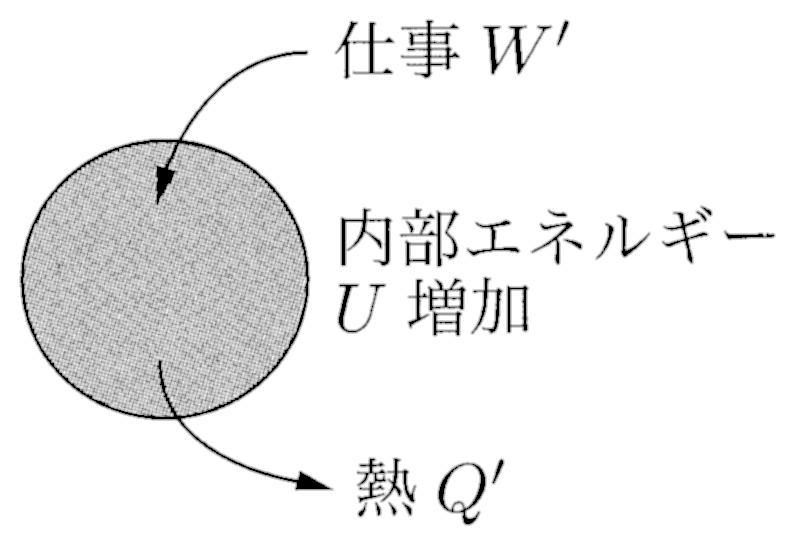
\includegraphics[keepaspectratio,width=38mm]{fig/ch14_p119_dU2.png}
       \end{center}
\end{komon}

\Rank{C問題}
\MonN{8}{状態方程式}\par\nopagebreak
\begin{sisin}
各状態において，各々の部分の圧力，体積，気体のモル数，温度がどのようになっているのかを考えて，$\mathrm{A}$内および$\mathrm{B}$内の状態方程式を立式し，これを整理せよ．

$\mathrm{A}$と$\mathrm{B}$は細管でつながれているが，$\mathrm{A}$と$\mathrm{B}$とに圧力差がある場合には圧力の高い方から低い方へと気体が移動してしまう．よって，\underline{定常状態においては}\hskip0pt\underline{$\mathrm{A}$と$\mathrm{B}$の}\hskip0pt\underline{気体の圧力は}\hskip0pt\underline{等しくなっている}．しかし，$\mathrm{A}$と$\mathrm{B}$との温度が等しいとは限らないことに注意．$\mathrm{A}$，$\mathrm{B}$の温度は独立に保つことができる．
\end{sisin}
\noindent{\gtfamily 【解答】}\par\nopagebreak
\hspace{1zw}$\mathrm{A}$，$\mathrm{B}$の体積を$V_0\U{m^3}$，気体定数を$R\U{J/mol\cdot K}$とする．$\mathrm{A}$と$\mathrm{B}$は細管でつながれているので，常に$\mathrm{A}$，$\mathrm{B}$内の気体の圧力は等しくなっている．
\begin{komon}
\ko{1} 今，コック$\mathrm{C}$を開いているので，$\mathrm{A}$，$\mathrm{B}$内の気体の圧力は外界の圧力$P_1$に等しくなっている．この状態における$\mathrm{A}$，$\mathrm{B}$それぞれの中にある気体のモル数を$n_0\U{mol}$とすると，状態方程式より
       \[\mathrm{A},\ \mathrm{B}:P_1V_0=n_0RT_1\]
       が成立する．この状態から，コック$\mathrm{C}$を開いたまま（＝$\mathrm{A}$，$\mathrm{B}$内の気体の圧力を$P_1$に保ったまま）$\mathrm{B}$の温度を$T_1$に，$\mathrm{A}$の温度を$T_0$にした．この変化後の$\mathrm{B}$の状態方程式は
       \[\mathrm{B}:P_1V_0=n_0RT_1\]
       のまま変わらないので，$\mathrm{B}$内の気体のモル数は$n_0$のまま変わらない．変化後の$\mathrm{A}$内の気体のモル数を$n_1\U{mol}$とすると，変化後の$\mathrm{A}$の状態方程式は，
       \[\mathrm{A}:P_1V_0=n_1RT_0\]
       となる．$\mathrm{B}$内の気体のモル数は不変ゆえ$\mathrm{A}$内の気体のモル数の変化のみ考えればよく，$\mathrm{A}$を冷却していく間に流入した気体のモル数（＝$\mathrm{A}$内の気体のモル数の増加量）は，
       \[\Delta n_{\mathrm{A}}=n_1-n_0\]
       であり，これがはじめ$\mathrm{B}$内にあった気体のモル数$n_0$の何倍となるかを求めると，
       \[\frac{\Delta n_{\mathrm{A}}}{n_0}=\frac{n_1-n_0}{n_0}=\frac{n_1}{n_0}-1\]
       \[=\frac{\dfrac{P_1V_0}{RT_0}}{\dfrac{P_1V_0}{RT_1}}-1=\frac{T_1}{T_0}-1\ \mbox{[倍]}\Ans\]
\ko{2} コック$\mathrm{C}$を閉じても$\mathrm{A}$と$\mathrm{B}$は細管でつながれているので，常に$\mathrm{A}$，$\mathrm{B}$内の気体の圧力は等しくなっている．よって，変化後の$\mathrm{A}$，$\mathrm{B}$内の気体の圧力は等しい．\par
       \hspace{1zw}また$\mathrm{A}$，$\mathrm{B}$の両方を温度$T_1$にするので，$\mathrm{A}$と$\mathrm{B}$は共通の圧力，温度を持つ．よって，$\mathrm{A}$，$\mathrm{B}$内に一様にムラなく気体が分布していると考えられるので，$\mathrm{A}+\mathrm{B}$を一つの一様な系とみなして状態方程式を立てることができる．$\mathrm{A}+\mathrm{B}$の体積$2V_0$の空間に，合計$n_1+n_0$の気体分子が，圧力$P_2$，温度$T_1$で広がっているので，
       \[P_2\cdot 2V_0=(n_1+n_0)RT_1\]
       \hspace{1zw}これと(1)の状態方程式の組み合わせにより，
       \[P_2=\frac{T_0+T_1}{2T_0}P_1\U{Pa}\Ans\]
\end{komon}

\MonN{9}{熱力学第二法則}\par\nopagebreak
\begin{sisin}
誘導に従う．熱力学第二法則が入試で問われることはまずないが，熱力学第二法則の二つの代表的な表現方法であるトムソンの原理，クラウジウスの原理については頭の片隅に置いておくとよい．
\end{sisin}
\noindent{\gtfamily 【解答】}\par\nopagebreak
\begin{list}{}{%
  \setlength{\leftmargin}{3zw}\setlength{\labelwidth}{1.5zw}%
  \setlength{\labelsep}{1zw}\setlength{\itemsep}{0pt}%
  \setlength{\parsep}{0pt}\setlength{\topsep}{2pt}\setlength{\partopsep}{0pt}}
\item[ア] F
\item[イ] D
\item[ウ] C（熱は自発的には高→低にしか流れない）
\item[エ] A
\item[オ] B（必ず一部分は熱を捨てる必要がある）
\item[カ] D
\item[キ] B
\item[ク] C（仕事であれば何に対してでも与えることが可能である）
\item[ケ] A（仕事も熱もエネルギーであるから，仕事という形態で高熱源にエネルギーを与えるのと，熱という形態で高熱源にエネルギーを与えるのとは何ら違いがない）
\item[コ] D
\item[サ] C
\end{list}

\end{multicols}
